\documentclass{article}
\usepackage[T1]{fontenc}
\usepackage{lmodern}
\usepackage{graphicx}
\usepackage{amsmath,amssymb}
\usepackage[a4paper,margin=2cm]{geometry}
\usepackage[absolute,overlay]{textpos}
\setlength{\TPHorizModule}{1mm}
\setlength{\TPVertModule}{1mm}
\usepackage[indonesian]{babel}
\usepackage{hyperref}
\setlength{\emergencystretch}{2em}
% unit: Halaman 7

\begin{document}

% === Halaman 7 (llm) ===

\vspace{80mm}

Sumber gambar: Kevin Tirtawinata, Studi dan Analisis Elliptic Curve Cryptography

% deskripsi: Grafik kurva eliptik dengan persamaan y^2 = x^3 - 10x + 13 pada koordinat Kartesius.
% bbox normalisasi: [0.3600, 0.3400, 0.6350, 0.8200]
\begin{textblock*}{57.75mm}(75.60mm,100.98mm)
\noindent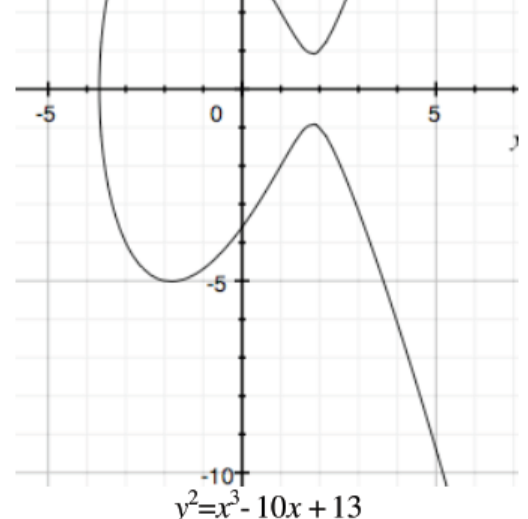
\includegraphics[width=57.75mm,height=142.56mm]{../../images/llm/page_007_img_01.png}%
\end{textblock*}

\end{document}
